\chapter{Results}

\section{Benchmarks Portfolios}
To inform our discussion of our agents' trading performance, we want to compare each of our benchmark portfolios against the S$\&$P 100 index performance.

\begin{center}
\begin{figure}
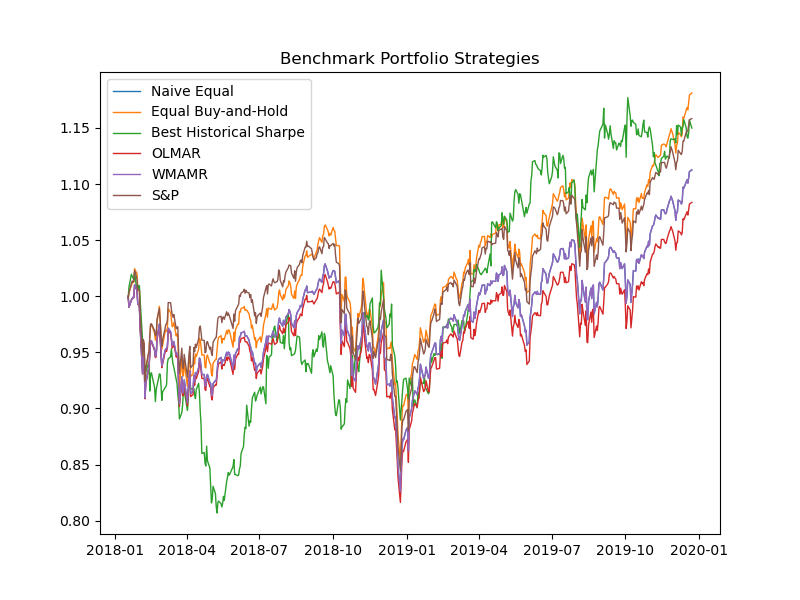
\includegraphics[width=.8\textwidth]{Benchmark Portfolio Strategies}
\end{figure}
\end{center}

\begin{table}[htbp]
    \centering
    \caption{Performance Metrics}
      \begin{tabular}{lcccc}
      \toprule
            & Net Profit & Sharpe Ratio & Sortino Ratio & Max Drawdown \\
      \midrule
      Naive Equal & 0.112583 & 0.392352 & -14.464945 & 0.197294 \\
      Equal Buy-and-Hold & 0.181138 & 0.595225 & -14.009800 & 0.198039 \\
      Best Historical Sharpe & 0.149857 & 0.475577 & -16.749871 & 0.210250 \\
      OLMAR & 0.083634 & 0.300906 & -14.344610 & 0.199240 \\
      WMAMR & 0.112565 & 0.392310 & -14.464168 & 0.197294 \\
      S\&P & 0.158347 & 0.552242 & -14.756129 & 0.197728 \\
      \bottomrule
      \end{tabular}%
    \label{tab:addlabel}%
  \end{table}%

As we can see, most of our benchmarks underperform the S$\&$P index over the trading period in terms of profitability. 
Further, the only benchmark that does outperform the S$\&$P (Naive Equal) has a significantly lower sharpe ratio (0.39) than the S$\&$P (0.55) indicating that after adjusting for portfolio deviation, the S$\&$P outperforms it.
Further, the maximum drawdown and sortino ratios for most of our benchmarks compared to the S$\&$P are fairly similar indicating that they have similar downside risks.

\section{RL Portfolios}
In this section, we describe the returns of our reinforcement learning agent portfolios in an environment including only historical price and returns data. We CNN, RNN, and MLP based policy networks and employ DDPG to optimize the policy.
We also test across each both of our rewards, differential sharpe ratio and profit.

\subsection{Differential Sharpe Reward}
\begin{table}[htbp]
    \centering
    \caption{Strategies with Historical Prices (Differential Sharpe Reward)}
      \begin{tabular}{lcccc}
      \toprule
            & Net Profit & Sharpe Ratio & Sortino Ratio & Max Drawdown \\
      \midrule
      Hist Prices CNN & 0.111205 & 0.396336 & -14.459686 & 0.199721 \\
      Hist Prices RNN & 0.069154 & 0.262906 & -14.991369 & 0.194177 \\
      Hist Prices MLP & 0.094686 & 0.338142 & -14.739489 & 0.188082 \\
      S\&P   & 0.158347 & 0.552242 & -14.756129 & 0.197728 \\
      \bottomrule
      \end{tabular}%
    \label{tab:addlabel}%
  \end{table}%

  \begin{center}
    \begin{figure}
    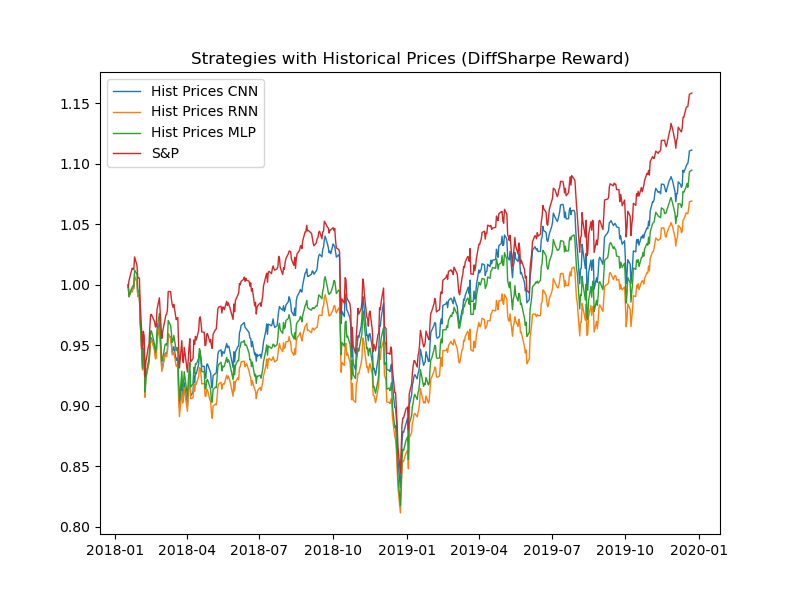
\includegraphics[width=.8\textwidth]{Strategies with Historical Prices (DiffSharpe Reward)}
    \end{figure}
    \end{center}

    \subsection{Profit Reward}

    \begin{table}[htbp]
        \centering
        \caption{Strategies with Historical Prices (Profit Reward)}
          \begin{tabular}{lcccc}
          \toprule
                & Net Profit & Sharpe Ratio & Sortino Ratio & Max Drawdown \\
          \midrule
          Hist Prices CNN & 0.166717 & 0.561471 & -14.923095 & 0.196557 \\
          Hist Prices RNN & 0.106518 & 0.369764 & -15.113139 & 0.205465 \\
          Hist Prices MLP & 0.071937 & 0.261355 & -15.265520 & 0.198329 \\
          S\&P   & 0.158347 & 0.552242 & -14.756129 & 0.197728 \\
          \bottomrule
          \end{tabular}%
        \label{tab:addlabel}%
      \end{table}%

    \begin{center}
        \begin{figure}
        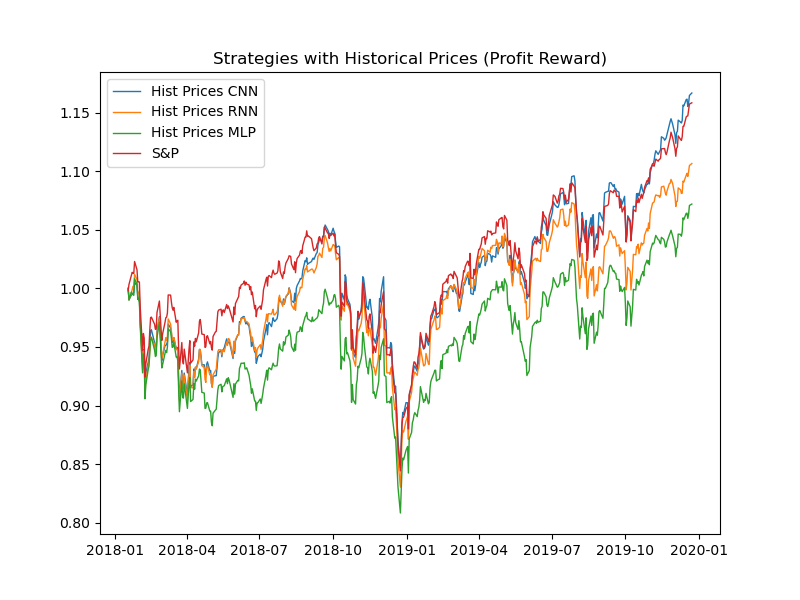
\includegraphics[width=.8\textwidth]{Strategies with Historical Prices (Profit Reward)}
        \end{figure}
        \end{center}

\section{RL Portfolio With Alternative Data}

\subsection{News Data}


\subsection{SEC Data}

\subsubsection{Differential Sharpe Reward}

\begin{table}[htbp]
    \centering
    \caption{Strategies with SEC Filings (Differential Sharpe Reward)}
      \begin{tabular}{lcccc}
      \toprule
            & Net Profit & Sharpe Ratio & Sortino Ratio & Max Drawdown \\
      \midrule
      SEC CNN & 0.124870 & 0.439863 & -14.397950 & 0.195347 \\
      SEC RNN & 0.138309 & 0.464039 & -14.439768 & 0.204159 \\
      SEC MLP & 0.147103 & 0.482788 & -14.519536 & 0.220906 \\
      S\&P   & 0.158347 & 0.552242 & -14.756129 & 0.197728 \\
      \bottomrule
      \end{tabular}%
    \label{tab:addlabel}%
  \end{table}%

\begin{center}
    \begin{figure}
    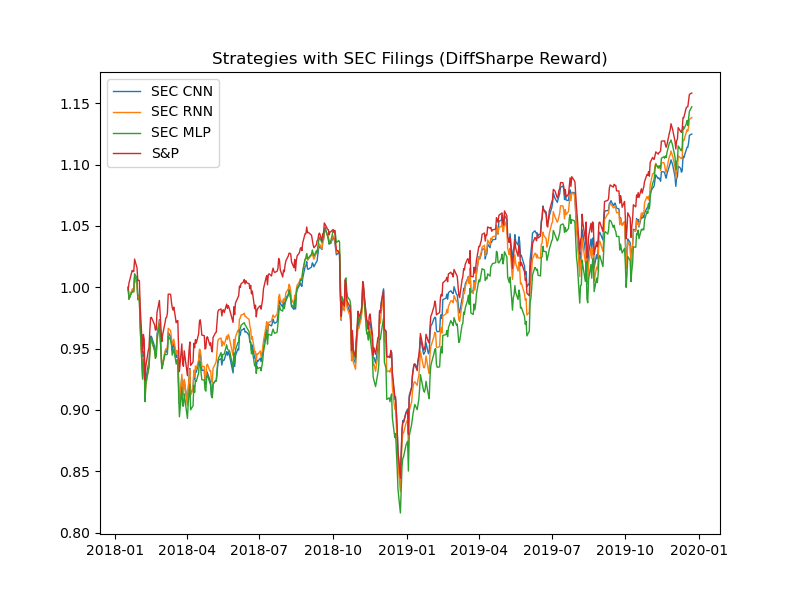
\includegraphics[width=.8\textwidth]{Strategies with SEC Filings (DiffSharpe Reward)}
    \end{figure}
\end{center}

\subsubsection{Profit Reward}

\begin{table}[htbp]
    \centering
    \caption{Strategies with SEC Filings (Profit Reward)}
      \begin{tabular}{lcccc}
      \toprule
            & Net Profit & Sharpe Ratio & Sortino Ratio & Max Drawdown \\
      \midrule
      SEC CNN & 0.162534 & 0.532298 & -14.478839 & 0.195766 \\
      SEC RNN & 0.154506 & 0.513757 & -14.728491 & 0.187671 \\
      SEC MLP & 0.073242 & 0.266018 & -15.909619 & 0.208675 \\
      S\&P   & 0.158347 & 0.552242 & -14.756129 & 0.197728 \\
      \bottomrule
      \end{tabular}%
    \label{tab:addlabel}%
  \end{table}%

\begin{center}
    \begin{figure}
    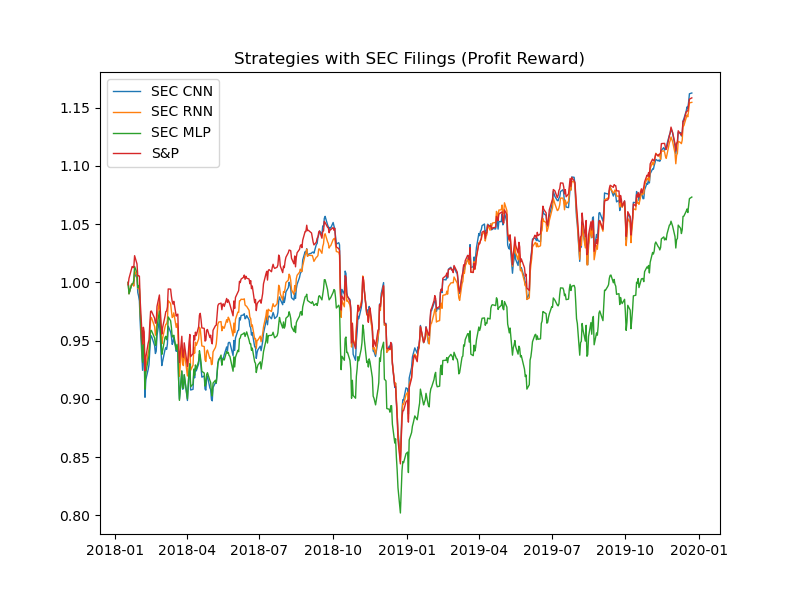
\includegraphics[width=.8\textwidth]{Strategies with SEC Filings (Profit Reward)}
    \end{figure}
\end{center}



\subsection{SEC and News Data Combined}

\subsubsection{Differential Sharpe Reward}

\begin{table}[htbp]
    \centering
    \caption{Performance Metrics of SEC+News Models and S\&P Benchmark}
      \begin{tabular}{lcccc}
      \toprule
            & Net Profit & Sharpe Ratio & Sortino Ratio & Max Drawdown \\
      \midrule
      SEC+News CNN & 0.094546 & 0.342485 & -14.805659 & 0.193996 \\
      SEC+News RNN & 0.128636 & 0.444354 & -14.533568 & 0.195274 \\
      SEC+News MLP & 0.053514 & 0.205204 & -15.149644 & 0.200069 \\
      S\&P   & 0.158347 & 0.552242 & -14.756129 & 0.197728 \\
      \bottomrule
      \end{tabular}%
    \label{tab:addlabel}%
  \end{table}%

  \begin{center}
    \begin{figure}
    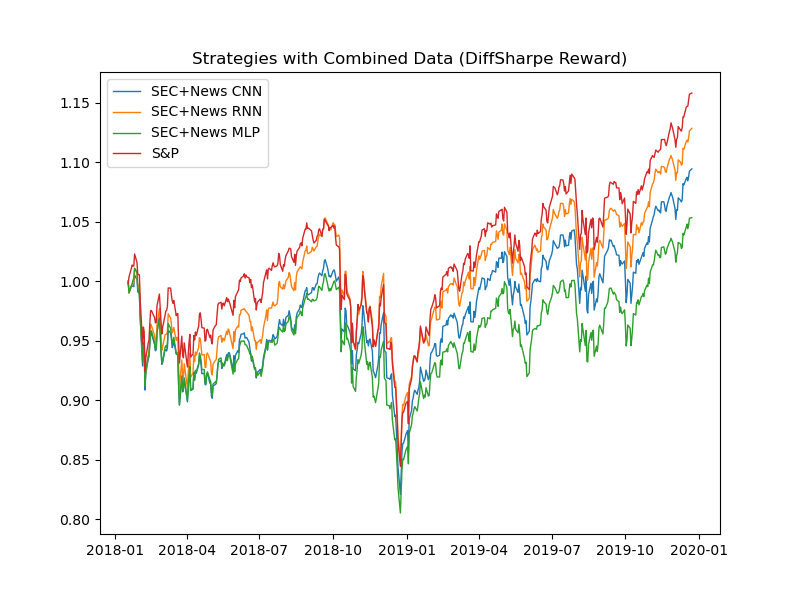
\includegraphics[width=.8\textwidth]{Strategies with Combined Data (DiffSharpe Reward)}
    \end{figure}
\end{center}

\subsubsection{Profit Reward}

\begin{table}[htbp]
    \centering
    \caption{Performance Metrics}
      \begin{tabular}{lcccc}
      \toprule
            & Net Profit & Sharpe Ratio & Sortino Ratio & Max Drawdown \\
      \midrule
      SEC+News CNN & 0.166081 & 0.553644 & -14.319155 & 0.195472 \\
      SEC+News RNN & 0.142287 & 0.519258 & -14.759413 & 0.170134 \\
      SEC+News MLP & 0.065676 & 0.248586 & -14.917642 & 0.195750 \\
      S\&P   & 0.158347 & 0.552242 & -14.756129 & 0.197728 \\
      \bottomrule
      \end{tabular}%
    \label{tab:addlabel}%
  \end{table}%

  \begin{center}
    \begin{figure}
    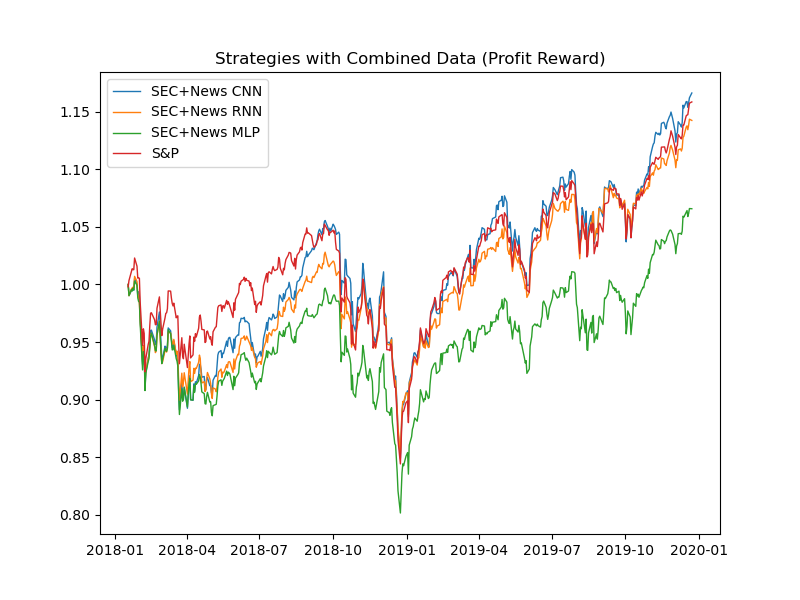
\includegraphics[width=.8\textwidth]{Strategies with Combined Data (Profit Reward)}
    \end{figure}
\end{center}


\section{Summary of Results}
Our principal observations indicate a disparity in learning complexity between the profit reward function and the differential Sharpe ratio for our agent, resulting in consistently superior portfolio performance when optimizing with the former. 
Notably, policy networks based on CNNs and RNNs exhibit enhanced performance under the profit reward, while the MLP policy network seems to overfit to S\&P returns.

Furthermore, our analysis underscores the challenge of integrating news data, revealing a diminished capacity of the model to learn the differential Sharpe ratio reward. We attribute this difficulty to the sparse and inconsistent nature of the dataset. However, it is noteworthy that the infusion of news data appears to minimally impact performance concerning the profit reward function, which again highlights the profit reward's relative simplicity.

Upon integrating SEC filings data, notable performance enhancements are observed across both reward functions compared to baseline models. Despite the sparsity of SEC filings, their regularity and consistency across all tickers facilitate improved learning for our policy algorithms, thus contributing to heightened performance.

Perhaps most intriguingly, optimal performance is achieved through hyperparameter tuning when integrating both news and SEC data into the states matrix. This outcome underscores the untapped potential of research avenues exploring comprehensive datasets capturing nuanced company sentiment.